\documentclass[11pt,a4paper]{report}
\usepackage{color}
% dasselbe Template wie Thesis mit nur leichten Anpassungen
% Nehmen Sie das Thesis-Template für die Thesis!
% Lesen Sie Hinweise zum Umgang mit LaTeX und zum Schreiben
% von Berichten im Thesis-Template nach
% => Moodle => PraxissemesterThesis => LaTeXThesis.zip
%    https://moodle.hs-mannheim.de/course/view.php?id=2500


% Für doppelseitigen Ausdruck (nur bei > 60 Seiten sinnvoll)
% \usepackage{ifthen}
% \setboolean{@twoside}{true}
% \setboolean{@openright}{true} 

% pakete
\usepackage{ifthen}

% Deutsch
\usepackage[german]{babel} % deutsch und deutsche Rechtschreibung
\usepackage[backend=biber, style=numeric, sorting=none]{biblatex} % Literaturverzeichnis (sortiert nach Reihenfolge des Auftretens)
\addbibresource{praksem.bib}
\usepackage[utf8]{inputenc} % Unicode Text
\usepackage[T1]{fontenc} % Umlaute und deutsches Trennen
\usepackage{textcomp} % Euro
% statt immer Ab\-schluss\-ar\-beit zu schreiben
% einfach hier sammeln mit -. 
\hyphenation{Ab-schluss-ar-beit}
% Vorsicht bei Umlauten und Bindestrichen
\hyphenation{Ver-st\"ar-ker-aus-gang}
 % eigene Hyphenations, die für das Dokument gelten
\usepackage{amssymb} % Symbole
\usepackage{emptypage} % Wirklich leer bei leeren Seiten

%% Fonts, je ein kompletter Satz an Optionen

% Times New Roman, gewohnter Font, ok tt und serifenlos
%\usepackage{mathptmx} 
%\usepackage[scaled=.95]{helvet}
%\usepackage{courier}

% Palatino mit guten Fonts für tt und serifenlos
\usepackage{mathpazo} % Palatino, mal was anderes
\usepackage[scaled=.95]{helvet}
\usepackage{courier}

% New Century Schoolbook sieht auch nett aus (macht auch tt und serifenlos)
%\usepackage{newcent}

% Oder default serifenlos mit Helvetica 
% ich kann es nicht mehr sehen ...
%\renewcommand{\familydefault}{\sfdefault}

% ein bisschen eine bessere Verteilung der Buchstaben...
\usepackage{microtype}

% Bilder und Listings
\usepackage{graphicx} % wir wollen Bilder einfügen
\usepackage{subfig} % Teilbilder
\usepackage{wrapfig} % vielleicht doch besser vermeiden
\usepackage{listings} % schöne Quellcode-Listings
% ein paar Einstellungen für akzeptable Listings
\lstset{basicstyle=\ttfamily, columns=[l]flexible, mathescape=true, showstringspaces=false, numbers=left, numberstyle=\tiny}
\lstset{language=python} % und nur schöne Programmiersprachen ;-)
% und eine eigene Umgebung für Listings
\usepackage{float}
\newfloat{listing}{htbp}{scl}[chapter]
\floatname{listing}{Listing}

% Seitenlayout
\newcommand{\seitenseitenabstand}{22mm} % 30mm
\usepackage[paper=a4paper,left=\seitenseitenabstand,right=\seitenseitenabstand,height=23cm]{geometry}
\usepackage{setspace}
% \linespread{1.15}
\linespread{1.1}
\setlength{\parskip}{0.5em}
\setlength{\parindent}{0em} % im Deutschen Einrückung nicht üblich, leider

% Seitenmarkierungen 
\newcommand{\phv}{\fontfamily{phv}\fontseries{m}\fontsize{9}{11}\selectfont}
\usepackage{fancyhdr} % Schickere Header und Footer
\pagestyle{fancy}
\renewcommand{\chaptermark}[1]{\markboth{#1}{}}
%\fancyhead[L]{\phv \leftmark}
\fancyhead[RH,LO]{\phv \nouppercase{\leftmark}}
\fancyhead[LH,RO]{\phv \thepage}
% Unten besser auf alles Verzichten
%\fancyfoot[L]{\textsf{\small \kurztitel}}
\fancyfoot[C]{\ } % keine Seitenzahl unten
%\fancyfoot[R]{\textsf{\small Technische Informatik}}

% Include subsubsections in the Table of Contents
% -1 for part
%  0 for chapter (only in report and book document classes)
%  1 for section
%  2 for subsection
%  3 for subsubsection
%  4 for paragraph
%  5 for subparagraph
\setcounter{tocdepth}{3}

% Theorem-Umgebungen
\newtheorem{definition}{Definition}[chapter]
\newtheorem{satz}{Satz}[chapter]
\newtheorem{lemma}[satz]{Lemma} % gleicher Zähler wie Satz
\newtheorem{theorem}{Theorem}[chapter]
\newenvironment{beweis}[1][Beweis]{\begin{trivlist}
                                       \item[\hskip \labelsep {\textit{#1 }}]}{
\end{trivlist}}
\newcommand{\qed}{\hfill \ensuremath{\square}}

%% Quellen
% Eine Alternative wäre Quellen in Literatur und Online-Quellen
% zu teilen
% \usepackage{bibtopic} 

% Hochschule Logo, noch nicht perfekt
\usepackage{hsmalogo}

% Spezialpakete
\usepackage{epigraph}
\setlength{\epigraphrule}{0pt} % kein Trennstrich

% damit wir nicht so viel tippen müssen, nur für Demo 
% \usepackage{blindtext}

% ifthen für sperrvermerk
\newif\ifsperrvermerk

% klickbare links im inhaltsverzeichnis
\usepackage{hyperref}
\hypersetup{
    colorlinks,
    citecolor=black,
    filecolor=black,
    linkcolor=black,
    urlcolor=black
}

% text shortcut variablen
\newcommand{{\metaeffekt}}{\{met\ae ffekt\}}
\newcommand{\bitkom}{bitkom}
\newcommand{\aeclientZEZESE}{Thales}
\newcommand{\headerand}{und\ }
% weekdays
\newcommand{\weekdayMondayLong}{Mo} % Mo, Montag
\newcommand{\weekdayTuesdayLong}{Di} % Di, Dienstag
\newcommand{\weekdayWednesdayLong}{Mi} % Mi, Mittwoch
\newcommand{\weekdayThursdayLong}{Do} % Do, Donnerstag
\newcommand{\weekdayFridayLong}{Fr} % Fr, Freitag
\newcommand{\weekdaySaturdayLong}{Sa} % Sa, Samstag
\newcommand{\weekdaySundayLong}{So} % So, Sonntag
\newcommand{\weekdayMondayShort}{Mo}
\newcommand{\weekdayTuesdayShort}{Di}
\newcommand{\weekdayWednesdayShort}{Mi}
\newcommand{\weekdayThursdayShort}{Do}
\newcommand{\weekdayFridayShort}{Fr}
\newcommand{\weekdaySaturdayShort}{Sa}
\newcommand{\weekdaySundayShort}{So}

% custom commands
\newcommand{\lweekdaymarginpar}[1]{%
    \marginpar{\raisebox{-1.6em}{\underline{#1}}}
}
\newcommand{\sweekdaymarginpar}[1]{%
    \marginpar{\raisebox{-1.92em}{\underline{#1}}}
}
\newcommand{\qt}[1]{„#1“}

\definecolor{codegray}{gray}{0.9}
\newcommand{\code}[1]{\colorbox{codegray}{\texttt{\detokenize{#1}}}}
\newcommand{\codendt}[1]{\colorbox{codegray}{\texttt{#1}}}

% custom environments
\newenvironment{smitemize}
{ \begin{itemize}
      \setlength{\itemsep}{0em}
      \setlength{\topsep}{0em}
      \setlength{\partopsep}{0em} }
      {
\end{itemize} }

% code listings
\input{latex-listings-powershell/src/latex-listings-powershell}
\definecolor{lst-gray}{rgb}{0.98,0.98,0.98}
\definecolor{lst-blue}{RGB}{40,0.0,255}
\definecolor{lst-green}{RGB}{65,128,95}
\definecolor{lst-red}{RGB}{200,0,85}
\lstset{
    commentstyle=\color{lst-green},
    basicstyle=\small\ttfamily,
    backgroundcolor=\color{lst-gray},
    breaklines=true,
    captionpos=b,
    columns=fixed,
    extendedchars=true,
    frame=single,
    framesep=2pt,
    keepspaces=true,
    keywordstyle=\color{lst-blue},
    language={PowerShell},
    numbers=left,
    numberstyle=\small\ttfamily,
    showstringspaces=false,
    stringstyle=\color{lst-red},
    tabsize=2,
}
 % alle Pakete und Einstellungen

% Hier anpassen 
\newcommand{\autor}{Yan Wittmann}
\newcommand{\matrikelnummer}{2121578}
\newcommand{\fachsemester}{5IB} % im wie vielten Semester waren Sie?
%\newcommand{\studiengang}{Medizintechnik}
%\newcommand{\studiengang}{Technische Informatik}
\newcommand{\studiengang}{Informationstechnik}
\newcommand{\firma}{\{metæffekt\} GmbH}
\newcommand{\standort}{Heidelberg}
\newcommand{\abteilung}{Automated Vulnerability Monitoring}
\newcommand{\betreuer}{Karsten Klein}
\newcommand{\pbeginn}{01.09.2023}
\newcommand{\pende}{29.02.2024}
\newcommand{\tage}{100} % arbeitstagerechner verwenden!
\newcommand{\titel}{Bericht zum praktischen Studiensemester}
\newcommand{\kurztitel}{Praxisbericht}
% \sperrvermerktrue % Kommentar am Anfang der Zeile löschen für Sperrvermerk

% Wenn jemand unbedingt ein Glossar will, die nächsten drei Zeilen...
%\usepackage{glossaries} % oder schlimmer mit [toc], damit es im TOC auftaucht
%\makeglossaries
%\newglossaryentry{Computer}{name=Computer,
    description={Eine programmierbare Maschine, die Eingaben erhält, Daten speichert und manipuliert
    und Ausgaben in einem sinnvollem Format ausgibt. (Und wer so was in ein Glossar eines Berichts
    für einen technischen Studiengang schreibt hat es nicht verstanden)}}
\newglossaryentry{naiv}{name=na\"{\i}ve,
description={Ein franzöisches Lehnswort (Adjektiv, Form von naïf)
Erweckt den Eindruch oder hat mangelnde Erfahrung, mangelndes Verständnis oder mangelnde Skills}}
\newglossaryentry{Linux}{name=Linux,
description={Generischer Ausdruck für eine Familie von Unix-artigen Betriebssystemen die den
Linux-Kernel verwenden},
plural=Linuces}
\newacronym[longplural={Frames per Second}]{fpsLabel}{FPS}{Frame per Second}
\newacronym{acme}{ACME}{A Company Making Everything}
\newglossaryentry{Praktisches Studiensemester}{name=Praktisches Studiensemester,
description={Im Rahmen des Ingenieursstudiums ein Semester in der betrieblichen Praxis
zur Ergänzung und Vertiefung des Studienwissens durch selbstständige ingenieurnahe Tätigkeit
betreut durch einen Ingenieur des Betriebes}}
 % In dieser Datei die Einträge definieren
% und noch ganz unten printglossaries auskommentieren
% Damit jetzt ein Glossar gezeigt wird noch \gls{label} verwenden

\begin{document}
    \begin{titlepage}
    \hsmalogo[1] \hfill
    \parbox[b]{60mm}{
        Fakultät Informationstechnik\\
        Studiengang \studiengang}
    \begin{center}
        \rule{1\textwidth}{1pt}\\[-3mm]
        \parbox[t][64mm]{110mm}{% 11 cm für Breite 13, ca. 7 für Höhe 6
            \Large{\ } \\[8mm]
            Bericht zum praktischen Studiensemester \\[4mm]
            \begin{tabular}{rl}
                \large{Vorgelegt von} & \large{\autor} \\[2mm]
                \large{Studiengang}   & \large{\studiengang} \\[2mm]
                \large{Firma}         & \large{\firma} \\[2mm]
            \end{tabular}
        }
        \rule{\textwidth}{1pt}
        \vfill
    \end{center}

    \vspace{2em}
    \begin{tabular}{ll}
        Name               & \autor                   \\
        Matrikelnummer     & \matrikelnummer          \\
        Studiengang        & \studiengang             \\
        Fachsemester       & \fachsemester \\[8mm]

        Praktikumszeitraum & \pbeginn\ \ bis \ \pende \\
        Präsenztage        & \tage \\[8mm]

        Firma              & \firma                   \\
        Standort           & \standort                \\
        Abteilung          & \abteilung               \\
        Betreuer           & \betreuer                \\
    \end{tabular}

    \vspace{8em}
    \noindent\begin{tabular}{p{0.48\textwidth}p{0.48\textwidth}}
                 \rule{0.46\textwidth}{0.5pt} & \rule{0.46\textwidth}{0.5pt} \\
                 Datum, \betreuer             & Firmenstempel
    \end{tabular}
    \vfill
\end{titlepage}
\cleardoublepage


% Erklärung gemäß der Prüfungsordnung
\thispagestyle{empty}
\subsection*{Selbstständigkeitserklärung}

Ich versichere, dass ich diesen Bericht zum praktischen Studiensemester
selbstständig und nur unter Verwendung der angegebenen Quellen und
Hilfsmittel angefertigt habe.
Die Stellen, an denen Inhalte aus den Quellen verwendet wurden, sind
als solche eindeutig gekennzeichnet.
Die Arbeit hat in gleicher oder ähnlicher Form bei keinem anderen
Prüfungsverfahren vorgelegen.

\vspace{6em}
\noindent\begin{tabular}{p{0.48\textwidth}p{0.48\textwidth}}
             \rule{0.42\textwidth}{0.5pt} & \rule{0.48\textwidth}{0.5pt} \\
             Datum, Ort                   & \makebox[1cm]{\ } \autor
\end{tabular}

\vfill

\ifsperrvermerk
\subsection*{Sperrvermerk}

Der vorliegende Bericht enthält interne und teilweise vertrauliche Daten
der Firma \newline \firma.
Der Bericht darf daher zu keinen anderen als Prüfungszwecken verwendet werden.
Insbesondere ist die Vervielfältigung und Veröffentlichung von Berichtinhalten
oder Teilen davon nur mit Zustimmung des Unternehmens erlaubt.
\vfill
\fi

\cleardoublepage

 % Titelseite, Erklärungen, etc.

    \begin{abstract}

        Abstract

    \end{abstract}

    \tableofcontents


    \chapter{Hintergrundinformation} \label{ch:hintergrund}


    \section{Firma} \label{sec:firma}


    \section{Team} \label{sec:team}


    \chapter{Einleitung} \label{ch:einleitung}


    %! Author = Yan Wittmann


\chapter{Tätigkeitsbeschreibung} \label{ch:wochenberichte}


% Einarbeitung in CVSS 4.0
\section{Woche 1 - Einarbeitung in CVSS 4.0} \label{sec:bericht-wo-1}

% Woche 1 (2023-09-04 bis 2023-09-08)

\lweekdaymarginpar{\weekdayMondayLong}

Mein erster Arbeitstag im Praktikums bei der {\metaeffekt} fiel mit dem Ende der Sommerpause des Unternehmens zusammen.
Da ich bereits seit einiger Zeit im Unternehmen arbeite und ich meine eigenständigen Aufgabenbereiche habe, war eine Einführung für mich nicht notwendig.
Bei {\metaeffekt} ist mein Aufgabenbereich als Entwickler ein automatisiertes Vulnerability Monitoring für unsere Kunden in der Programmiersprache Java zu implementieren und zu betreuen.
Als Hauptverantwortlicher für dieses Gebiet bin ich darüber hinaus für den Kundenkontakt für Fragen, Anforderungen und Unterstützung zuständig.
Ich verbrachte den Montag damit, einige während der Sommerpause aufgetretene Fehler in den Systemen von Kundenprojekten zu korrigieren und Gespräche mit Kollegen zu führen, um anstehende Projekte und Aufgaben zu klären.

Ein wichtiges Thema war die anstehende Veröffentlichung des CVSS 4.0-Standards, die für den 31.\ Oktober 2023\footnote{\url{https://www.first.org/cvss/v4-0/}} geplant war.
Die Software-Implementierung der {\metaeffekt} ist bereits in der Lage, die Scores der CVSS-Versionen 2.0 und 3.1 zu berechnen, und wir müssen in der Lage sein, auch die neuen CVSS 4.0-Vektoren zu berechnen, sobald offizielle Datenquellen diese auch bei sich integrieren.
Mit meinem Chef und Betreuer für das Praktikum, Karsten Klein, habe ich zudem vereinbart, während meines Praxis-Semesters tägliche Meetings mit ihm abzuhalten.

\sweekdaymarginpar{\weekdayTuesdayLong}

Am Dienstag startete ich damit, die zu dem Zeitpunkt noch unfertige Dokumentation und Beispiele von CVSS 4.0 zu studieren.
Ich stellte schnell fest, dass es mehr Unterschiede als Gemeinsamkeiten zu den vorherigen Versionen gibt, insbesondere in Bezug auf die mathematischen Hintergründe.
Ich dokumentierte dennoch meine Erkenntnisse in unserem internen Confluence Wiki.
Auf dem offiziellen RedHat GitHub-Repository\footnote{\url{https://github.com/RedHatProductSecurity/cvss-v4-calculator}} fand ich den Quellcode einer Referenz-JavaScript-Implementierung, die noch sehr nützlich werden sollte.

\sweekdaymarginpar{\weekdayWednesdayLong}

Am Mittwoch begann ich mit einem ersten Versuch einer Implementierung der CVSS 4.0-Berechnungen.
Wie ich bereits gestern vermutet hatte, ist die Berechnung bei 4.0 mathematisch deutlich komplexer, mit Hamming-Distanzen zwischen Vektoren und der Interpolation und Skalierung von mehrdimensionalen Räumen, versehen.
Dank der RedHat JavaScript-Implementierung konnte ich Mittwoch das Grundgerüst für meine Implementierung in Java vorbereiten.

\sweekdaymarginpar{\weekdayThursdayLong}

Der Donnerstag startete mit der Behebung einer \qt{OutOfMemoryError}-Exception im Code eines unserer Reports in einem Kundenprojekt, die auftrat, wenn eine zu große Menge an Daten verarbeitet wurde.
Das Problem war, dass während der Serialisierung in ein HTML-Dokument das interne Modell (damit auch der Speicherbedarf) kurzzeitig dupliziert wurde.
Ich konnte das Problem lösen, indem ich einen FileAppender verwende, der den HTML-String des Reports direkt in eine Datei schreibt, anstatt ihn wie zuvor im Speicher zu halten.

Der Hauptteil meines Tages war jedoch der Untersuchung von CVSS 4.0 zugeordnet.
Leider musste ich im Verlauf feststellen, dass die Referenzimplementierung und die Spezifikation im aktuellen Zustand voneinander abweichen, was bei einem unveröffentlichten Standard zwar verständlich, aber nicht hilfreich ist.
Ich meldete dieses Problem zusammen mit inhaltlichen Fragen in einem GitHub-Issue\footnote{\url{https://github.com/RedHatProductSecurity/cvss-v4-calculator/issues/32}} und beendete den Tag mit einer teilweise funktionierenden Implementierung.

\sweekdaymarginpar{\weekdayFridayLong}

Am Freitag erhielt ich recht schnell eine Antwort auf meine Fragen:
Wie erwartet ist die Spezifikation veraltet und die Implementierung korrekt.
Mithilfe dieser Informationen konnte ich die Berechnungen fertigstellen und durch einen Test-Datensatz, den ich durch die Referenzimplementierung erzeugt habe, validieren.
Damit war der erste Teil dieses Tasks erledigt:
Als Nächstes wollte ich mein Verständnis für die Theorie hinter CVSS 4.0 verbessern und zudem musste die neue Version noch richtig in unsere Systeme integriert werden.

Freitagmittag findet bei der {\metaeffekt} ein wöchentliches Meeting statt, das als \qt{Weekly} bezeichnet wird.
Hier berichtete ich über meine Erfahrungen mit der Implementierung von CVSS 4.0 und hörte, was die anderen Teammitglieder in dieser Woche erreicht hatten.
So beendete ich meine erste Praktikumswoche.


% Vertiefung in CVSS 4.0 und Korrelationsdaten
\section{Woche 2 - Vertiefung in CVSS 4.0 \headerand Korrelationsdaten} \label{sec:bericht-wo-2}

\lweekdaymarginpar{Montag}
Die zweite Woche meines Praktikums wollte und sollte ich mich mit der genaueren Funktionsweise von CVSS 4.0 auseinandersetzen.
Ich verbrachte also den Montag damit, die Spezifikation\footnote{\url{htthttps://www.first.org/cvss/v4.0/specification-document}},
die Entwicklungsgeschichte\footnote{\url{https://www.first.org/cvss/v4.0/user-guide#New-Scoring-System-Development}}
und den Code tiefergehender anzusehen, um zu verstehen, wie die Berechnung des Scores funktioniert.

Ich hatte bereits während der Implementierung einen guten Überblick über den ersten Schritt der Berechnung, den mit den MacroVektoren, erhalten.
Die Unklarheiten lagen eher in dem zweiten Schritt: Der Interpolation zwischen den MacroVektor-Blasen.
Ich konnte selbst nach einem ganzen Tag an Recherche keine zufriedenstellende Erklärung finden, wie die Berechnung in diesem Schritt funktioniert.
Durch meine Recherche konnte ich immerhin weitere Randfall-Tests anlegen und damit zwei Fehler in meiner Implementierung finden.

\sweekdaymarginpar{Dienstag}
Eigentlich wollte ich am Dienstag weiter an meinem Verständnis von CVSS 4.0 arbeiten, aber es gab etwas Wichtigeres:
Da ein Kollege noch im Urlaub war, musste ich einen Teil seiner Arbeit übernehmen.
Es geht um das Pflegen von Korrelationsdaten, die dazu dienen, Software-Komponenten automatisch zu Produkten in fremden Datenbanken (wie den CPE in der NVD\footnote{\url{https://nvd.nist.gov/products/cpe}}) zuzuordnen.
Da dies früher einmal meine Aufgabe im Unternehmen war, habe ich dafür in der Vergangenheit ein Tool geschrieben, das ich kurz vor meinem Praktikum mit viel Feedback von und für meinen Mitarbeiter als Web-UI neu aufgesetzt hatte.
Das gab mir also die Chance, dieses Tool endlich einmal selbst zu verwenden und an einigen Stellen den Workflow zu verbessern.

\sweekdaymarginpar{Mittwoch}
Leider war ich Dienstag nicht mit den zu verarbeitenden Korrelationsdaten fertig geworden, darum habe ich noch den halben Mittwoch damit verbracht.
Was mich positiv überraschte war, wie gewissenhaft mein Kollege diese Arbeit durchgeführt hatte, seitdem er diese von mir übernommen hatte.
Ich musste nur bei wenigen Einträgen die Matching-Informationen überarbeiten, bei den meisten hatten diese bereits gestimmt und ich musste sie nur noch abnicken.

Den restlichen zwei Stunden habe ich dann noch mit meinem Chef über ein interessantes Thema reden können: Dem Abbilden von Vulnerability Chaining in unseren Systemen.
Also: was passiert, wenn man eine kritische Software-Schwachstelle, die man zuvor als \qt{Nicht Ausnutzbar} abgestempelt hatte, über eine andere, für sich alleine stehende harmlose, Schwachstelle ausnutzen kann?
Dieses Thema müssen wir auf Kundenwunsch in den nächsten Monaten abbilden können, aber eine hohe Priorität bekommt es noch nicht.

\sweekdaymarginpar{Donnerstag}
Donnerstag war mein Chef nicht im Büro, da er ein Treffen bei einem Kunden hatte.
Es war auch ein Tag, an dem ich sehr viel Code geschrieben habe, denn ich musste meine Planung für die Woche etwas umpriorisieren:
Ende der Woche musste die Implementierung und Integration von CVSS 4.0 in unser System fertiggestellt sein, darum beschloss ich, mich erst einmal darum zu kümmern und danach erst weiter mein Verständnis aufzubauen.
Die folgenden Punkte mussten bearbeitet werden:

\begin{smitemize}
    \item das Parsing der Vektoren aus verschiedenen Datenquellen/Formate (intern, extern)
    \item das korrekte Verarbeiten, wenn es um die Berechnung von Scores, das Modifizieren von Vektoren, oder das Ablegen in unseren Software-Inventaren geht
    \item das Anzeigen der Ergebnisse in unseren HTML- und PDF-Reports
\end{smitemize}

Da die externen Datenquellen ja noch keine Vektoren für CVSS 4.0 herausgeben, musste ich einige Annahmen über deren Formate machen, die ich bei tatsächlicher Veröffentlichung dann noch anpassen werde.

Bei diesen Arbeiten sind mir erst einige merkwürdige Muster in der Implementierung für die Berechnung der Scores aufgefallen, die ich mehr oder weniger aus der Referenz-Implementierung übernommen hatte.
Ich habe also fast noch einmal die gesamte Implementierung neu geschrieben, indem ich duplizierten Code in eigene Methoden und Klassen extrahiert und die Berechnungen wesentlich eleganter und näher an den dahinterliegenden mathematischen Modellen in meinem Programm abgebildet habe.

Am Ende des Tages hatte ich Pull Requests für die drei Projekte, in denen diese Berechnungen stattfinden, fertiggestellt.

\sweekdaymarginpar{Freitag}
Der Freitag begann frostig - im wahrsten Sinne des Wortes.
Es waren nur 7 °C und mit dem Fahrrad und kurzer Hose bin ich gut durchgefroren angekommen.
Mit einem Tee konnte ich mich aber ganz gut wieder aufwärmen.

Da ich die Integration bereits Donnerstag fertiggestellt hatte, habe ich mich wieder an das Verständnis über den CVSS 4.0 Standard gesetzt.
Um besser verstehen zu können, wie die MacroVektor Interpolation funktioniert, habe ich mir drei Beispiele herausgesucht und die Berechnungen aufgrund der Spezifikation und meiner Implementierung manuell mehrfach auf verschiedene Arten durchgeführt.
Das hat tatsächlich sehr geholfen und kurz vor dem Weekly hatte ich dann ein ganz gutes Verständnis, wie die Berechnung funktioniert.
Dies habe ich in einem Dokument für späteren Zugriff festgehalten.

Das Weekly war stark gefüllt, nicht nur ich hatte viele Neuigkeiten über die Funktionsweise von CVSS 4.0 zu berichten, sondern zwei meiner Kollegen hatten diese Woche auch in ihren Teilprojekten größere Durchbrüche, die sie sogar live demonstriert und erklärt haben.
Damit wurde das Weekly von einer Stunde auf fast zweieinhalb Stunden verlängert und der Tag war schnell herum.
Ich beendete meine zweite Woche mit einem guten Gefühl, diese Woche viel geschafft zu haben.


% Excel-Limitierungen & Präsentationsvorbereitung
\section{Woche 3 - Excel-Limitierungen \headerand Präsentationsvorbereitung} \label{sec:bericht-wo-3}

% Woche 3 (2023-09-18 bis 2023-09-24)

\lweekdaymarginpar{Montag}
Der Montag verlief eher ruhig, es gab keine größeren Themen, die dringend anstanden.
Darum lag mein Fokus daran, endlich einmal einige der Issues aus dem Jira-Backlog abzuarbeiten, die schon zu lange nötig waren.

Bei einem dieser Issues ging es darum, in unserem automatisierten CPE Matching-Algorithmus zwischen Hardware- und Software-Komponenten zu unterscheiden.
Dadurch würden wesentlich weniger false-positives entstehen, weil keine Softwarekomponenten mehr Hardware-CPEs zugeordnet werden würden.
Dazu war erst einmal eine Liste an Kategorien für Hardware nötig, die für die einzelnen Komponenten vergeben werden können.

Das Problem hierbei war der Detailgrad der Kategorien, welcher noch nicht festgelegt wurde.
Ich habe also nach einiger Recherche drei Vorschläge vorbereitet, die ich meinem Chef präsentierte.
Mein Chef und ich konnten uns recht schnell auf einen einigen, allerdings wollten wir uns noch eine Drittmeinung von einem Kollegen einholen.
Dieser hatte zu diesem Thema deutliche andere Meinungen, wie eine solche Liste auszusehen hatte.

Die Diskussion hierüber hat den gesamten restlichen Tag eingenommen und leider konnten wir bei keinem Ergebnis landen, mit dem alle zugestimmt hätten.
Wir machten aus, diese Diskussion an einem anderen Tag fortzuführen und damit war das Ende des Tages für mich erreicht.

\sweekdaymarginpar{Di, Mi, Do}

Die folgenden Tage konnte ich mich an etwas setzen, was ich schon lange in unserem Core-Projekt angehen wollte:
Es geht um die Serialisierung und Deserialisierung unserer Software-Inveterate zu Excel-Dateien.
Zellen speziell in Excel-Dokumenten haben ein Zeichenlimit von $32.767$\footnote{\url{https://support.microsoft.com/en-gb/office/excel-specifications-and-limits-1672b34d-7043-467e-8e27-269d656771c3}}, was in vielen unserer Fälle nicht ausreicht.
Seitdem ich bei der {\metaeffekt} bin, haben wir einen Workaround verwendet, der bereits in unserem Datenmodell nach einem System diese Zellen in mehrere Zellen aufteilt, sodass beim Serialisieren keine Probleme auftreten.
Das führt dazu, dass man nicht einfach so auf die betroffenen Felder in unserem Modell zugreifen kann, ohne speziell von dem Workaround Gebrauch zu machen.

Dass dies keine schöne Lösung ist, muss ich nicht erst sagen.
Probleme daran sind zum Beispiel:

\begin{smitemize}
    \item weiß jemand nicht von diesem Workaround, bekommt er vielleicht nur einen Bruchteil seiner Daten, wenn er die falsche Zugriffsart verwendet
    \item das Stylen der Excel-Zellen und Spalten funktioniert nicht richtig, da die Spalten aufgeteilt werden
    \item falls ein anderes Format mit niedrigerem Limit hinzugefügt werden soll, muss dieses Limit auch bei allen anderen Formaten so angewendet werden
\end{smitemize}

Ich war also recht froh, dass ich mich endlich einmal daran setzen konnte.
Ich habe die drei Tage nicht nur dazu genutzt, die Spaltung der Spalten in die Serialisierer zu verschieben, sondern auch ein allgemeines Styling-Modell einzuführen, das unabhängig vom Format auf Serialisierte Daten angewendet werden kann und einfach auf neue Formate angepasst werden kann.

\sweekdaymarginpar{Freitag}
Freitagmorgen wurde ich von meinem Chef erst einmal überrascht:
Nächste Woche Dienstag und Mittwoch sollte mit ihm und einer Kollegin nach Erfurt auf das Treffen des Arbeitskreises OpenSource\footnote{\url{https://www.bitkom.org/Bitkom/Organisation/Gremien/Open-Source.html}} unter dem Thema \qt{Open-Source-Communities} und das Forum OpenSource\footnote{\url{htthttps://www.bitkom.org/bfoss23}} der Bitkom gehe.

So weit, so gut.
Danach kam allerdings etwas, das ich nicht erwartet hätte: Ich sollte bei dem Treffen des Arbeitskreises OpenSource eine 25-Minütige Präsentation vor 30 Leuten von RedHat, Siemens, DB Systel und anderen großen Unternehmen über \qt{Identifikation und Bewertung von Schwachstellen mit Inhalten aus öffentlichen Quellen} halten.

Das kam überraschend, da ich noch nie auf einem solchen Treffen war und keine Ahnung hatte, wie eine solche Präsentation auszusehen hat.
Zum Glück hat mir mein Chef am Freitag noch geholfen, die wichtigen Themen aufzulisten und in eine sinnvolle Reihenfolge zu bringen.
Ich habe jedoch schnell gemerkt, dass die Zeit am Freitag und Montag nicht reichen werden, um die Präsentation vorzubereiten.
Ich habe zwar den Foliensatz an diesem Tag noch größtenteils fertigstellen können, aber das Skript hatte ich gerade erst angefangen zu verfassen.

\sweekdaymarginpar{Sa, So}
Und so kam das erste Mal, dass ich an einem Wochenende für die {\metaeffekt} gearbeitet habe.
Ich verbrachte das gesamte Wochenende damit, ein 11-seitiges Skript vorzubereiten, das alles enthält, was ich unbedingt in der Präsentation erwähnen wollte.
Natürlich habe ich die Präsentationsfolien weiter angepasst und mir Punkte notiert, die ich noch mit meinem Chef am Montag besprechen wollte.
Am Sonntagabend hatte ich dann ein Skript, mit dem ich zwar zufrieden war, aber irgendwie noch etwas fehlte.


% AK OpenSource & OpenSource Forum Erfurt
\section{Woche 4 - AK OpenSource \headerand OpenSource Forum Erfurt} \label{sec:bericht-wo-4}

% Woche 4 (2023-09-25 bis 2023-09-29)

\lweekdaymarginpar{Montag}

Nach einer kurzen Nacht, in der ich die letzten Feinschliffe an meinem Präsentationsskript anwendete, besprach ich Montag mit meinem Chef noch die letzten Unklarheiten.
Eines meiner Probleme bis jetzt war ein spezifischer Teil der Präsentation, der über ein Thema ging, mit dem sich zwar mein Chef gut auskennt, ich allerdings sehr wenig.
Mein Chef übernahm glücklicherweise kurzerhand diesen Teil.
Den Rest des Tages nutzte also ich lieber im Home-Office, um in Ruhe die Präsentation zu üben und meine Reisetasche für die morgige Reise nach Erfurt zu packen.

\sweekdaymarginpar{Dienstag}

Der Dienstag begann früh mit unserer Reise mit dem ICE nach Erfurt.
Während der Zugfahrt nutzten mein Chef und ich die Zeit für eine letzte Durchsprache unserer Präsentation.
Angekommen in Erfurt ging es direkt in den nahegelegenen Räumlichkeiten der DB Systel.
Dort gab es zunächst einige einleitende Worte und eine Vorstandswahl, bevor ich mit meiner Präsentation dran war.

Meine Kollegen vor Ort haben mich noch einmal ermutigt und trotz anfänglicher Nervosität verlief alles reibungslos:
Ich war gut vorbereitet, hatte die Präsentation gut geübt und die Themen, die ich vorstellte, gehören zu meinem täglichen Arbeitsbereich seit drei Jahren.
Ich brauchte mein Skript kaum und das Feedback war ausschließlich positiv, was mich sehr gefreut hat, denn ich wollte wirklich einen Mehrwert in diese Runde bringen.

Abends wurde vom {\bitkom} eine Stadtführung und ein gemeinsames Abendessen mit anderen Teilnehmern des OpenSource Forums des nächsten Tages organisiert, an welchen wir teilnahmen.
Dort, und bereits beim Arbeitskreis, konnten wir uns auch mit den anderen Teilnehmern austauschen.

\sweekdaymarginpar{Mittwoch}

Das OpenSource Forum der {\bitkom} bot dann eine entspannte Alternative zum vorherigen Tag, bei dem die Teilnehmer vielfältige Präsentationen verfolgen und sich untereinander auszutauschen konnten.
Besonders spannend waren die Einblicke in die Open-Source-Strategien großer Unternehmen wie SAP, Siemens und Mercedes.
Die Parallelen im Bezug auf die aktuellen Herausforderungen und Lösungsansätze für die Verwaltung von Schwachstellen und Lizenzen von Open-Source-Software in ihren Produkten und Projekten haben mich etwas überrascht und bestätigten die Relevanz unserer Arbeit.

\begin{figure}[htbp] % here, top, bottom, separate page
    \centering
    \includegraphics[width=0.5\textwidth, keepaspectratio]{res/img/2023-10-19-yan-ak-os}
    \caption{Auf dem Forum Open Source der Bitkom 2023}
    \label{fig:foss23-yan}
\end{figure}

Ein großer Programmpunkt war auch der {\bitkom} OpenSource Monitor\footnote{\url{https://www.bitkom.org/opensourcemonitor2023}}, den die {\metaeffekt} gesponsert hat und damit einen Beitrag über den Cyber Resilience Act\footnote{\url{https://digital-strategy.ec.europa.eu/en/policies/cyber-resilience-act}} in diesem verfassen durfte.
Wir wurden auch auf der großen Leinwand aufgeführt, wie in Abbildung\ \ref{fig:foss23-sponsor-metaeffekt} zu sehen ist.

\begin{figure}[htbp] % here, top, bottom, separate page
    \centering
    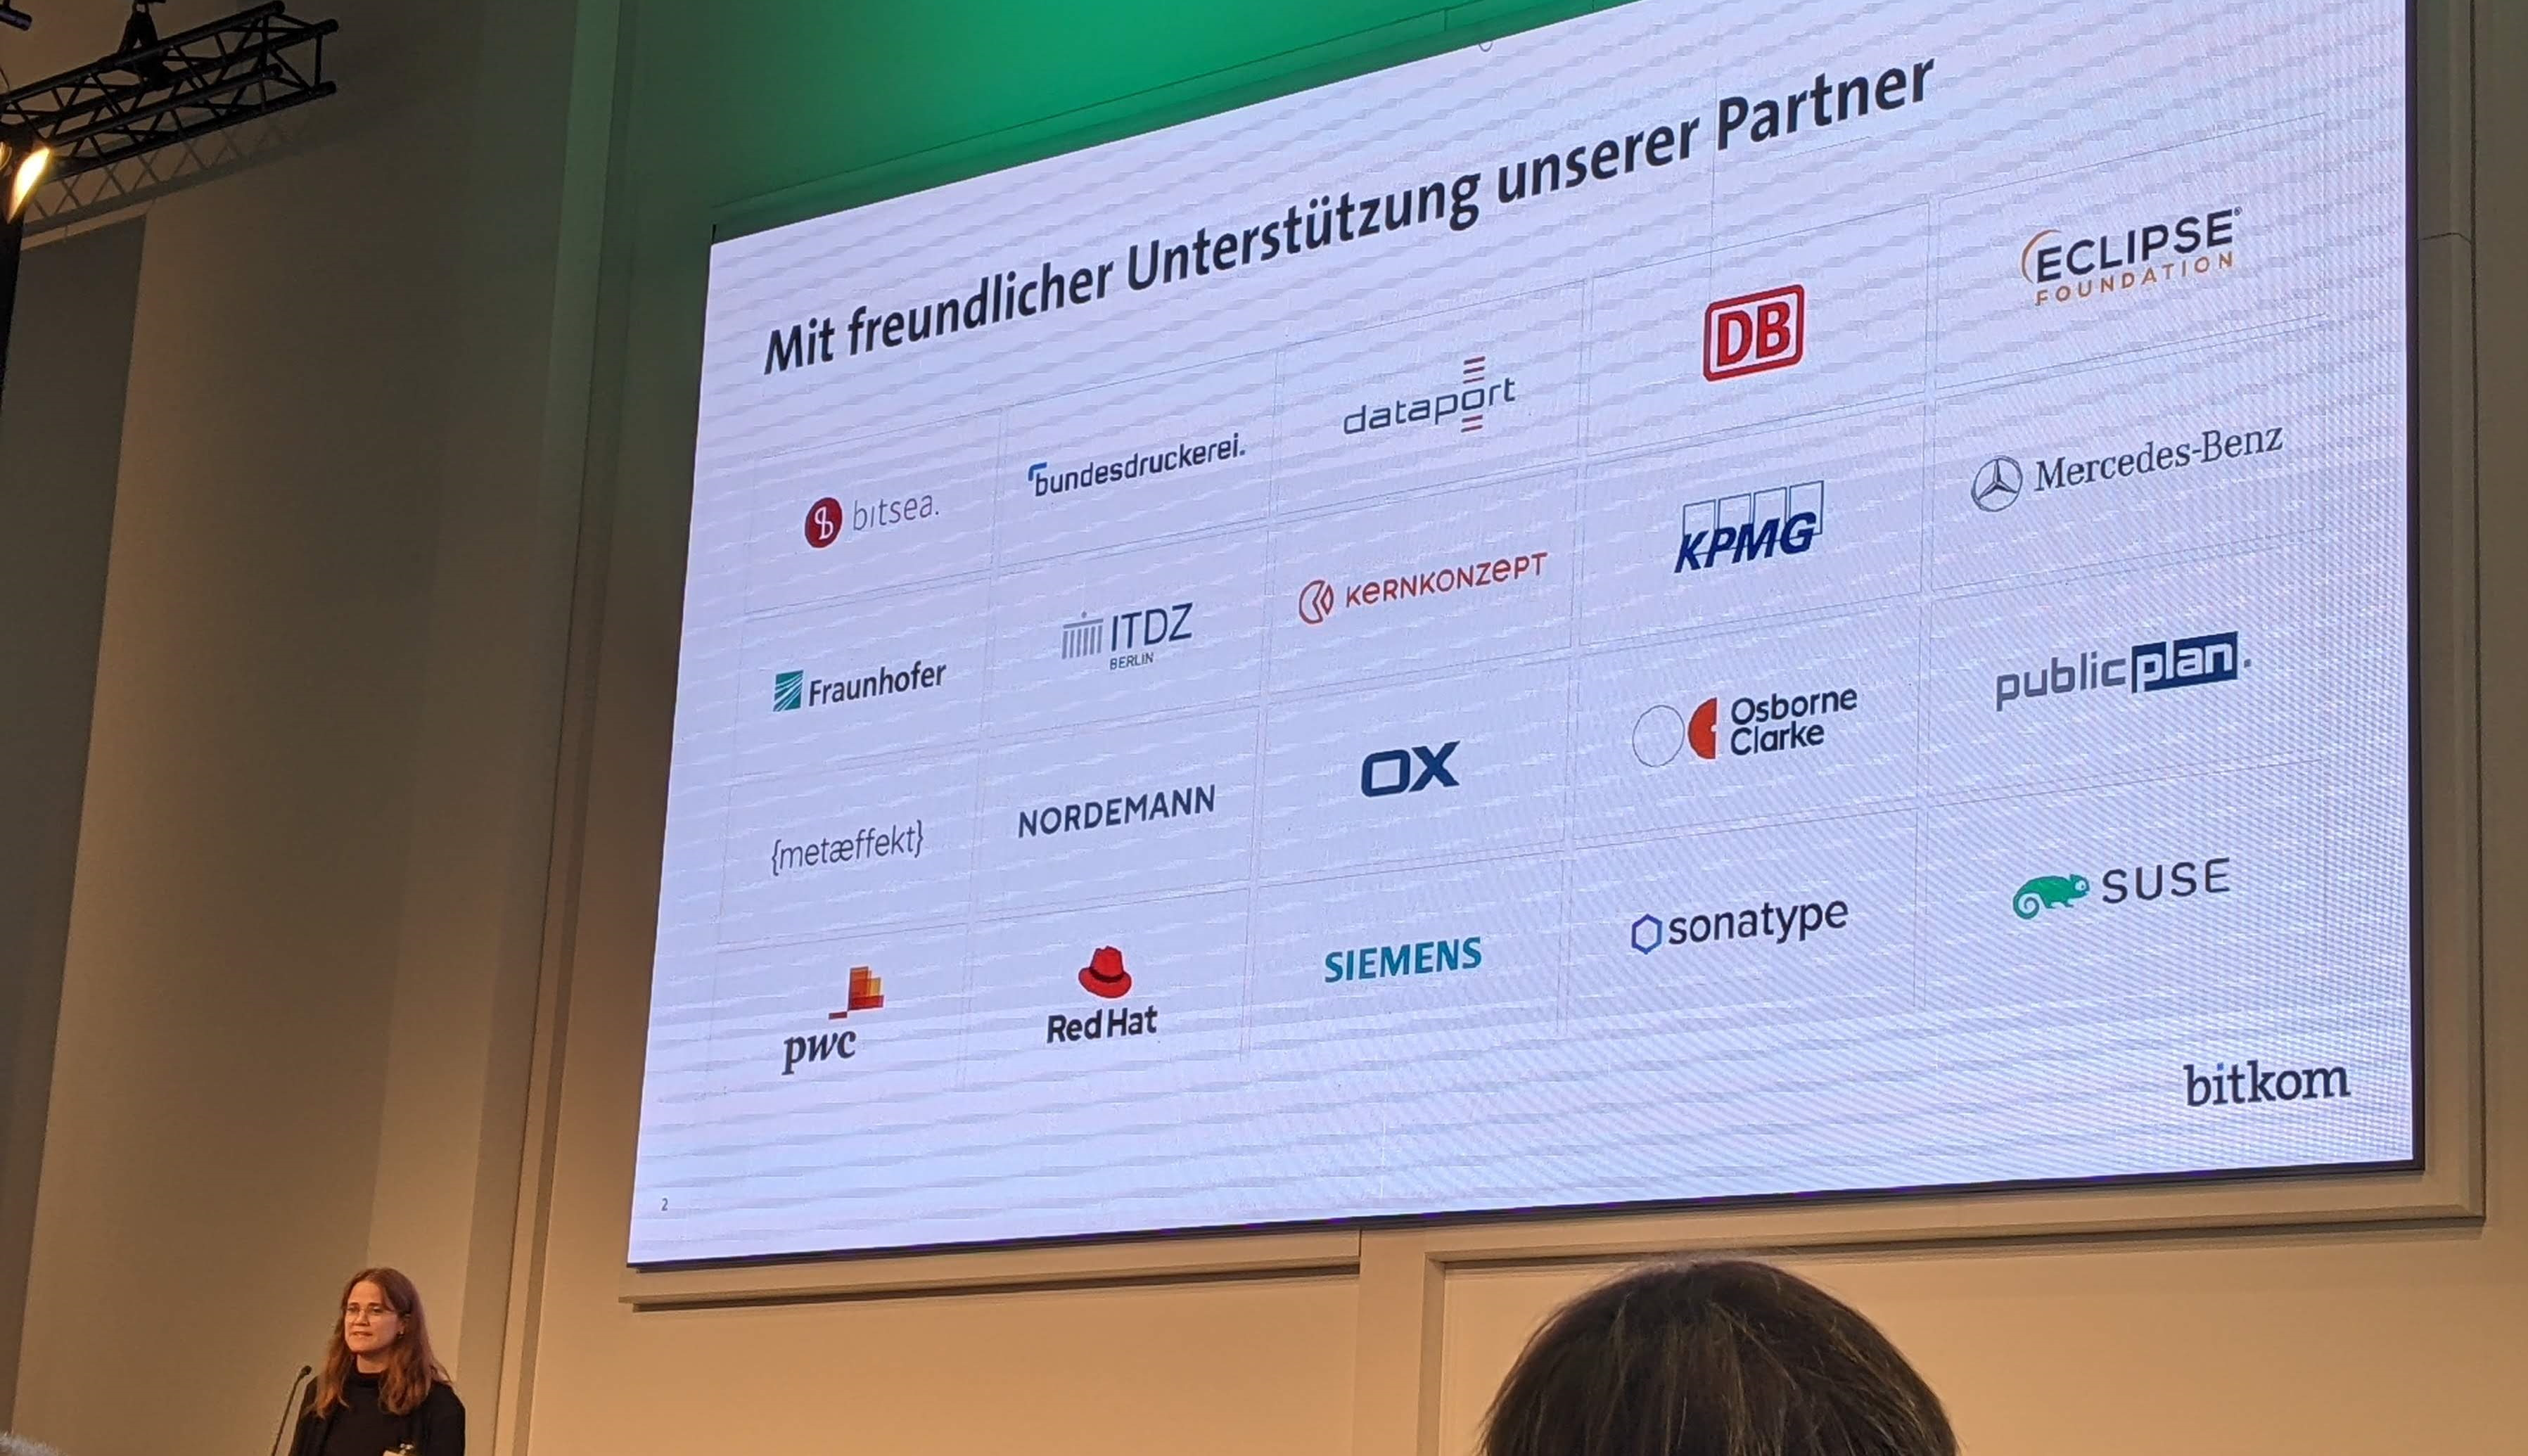
\includegraphics[width=0.8\textwidth, keepaspectratio]{res/img/2023-10-19-ak-os-metaeffekt-sponsor}
    \caption{Die {\metaeffekt} ist links als Sponsor zum OpenSource Monitor aufgeführt}
    \label{fig:foss23-sponsor-metaeffekt}
\end{figure}

Es gab einige bekannte Gesichter vom vorherigen Tag, aber auch einige unserer direkten Kunden waren vertreten, die ich noch nie in Person getroffen hatte.
Außerdem hatte ich die fantastische Chance direkt mit Studenten und Angestellten verschiedener Unterehen zu sprechen.

\sweekdaymarginpar{Do, Fr}

Die Rückreise am Donnerstag verlief ohne Zwischenfälle, sodass der Freitag wieder der gewöhnliche Arbeitsalltag war.
Eine neue Kundenanforderung erforderte schon wieder meine direkte Aufmerksamkeit:
Einer unserer Download-Prozesse scheitert in ihrer Konfiguration, da der verwendete git-Befehl die konfigurierte Proxy-Informationen bislang scheinbar ignoriert.
Um das zu lösen, kann Git sowohl über Umgebungsvariablen konfiguriert werden, als auch über einen Konfigurationsparameter im Befehlsaufruf.
Ich habe mich für die Umgebungsvariablen entschieden, die ich in der Prozess-Session, die über Java geöffnet wird, mit den Proxy-Informationen setzen kann.

Ein persönliches Highlight war diesen Freitag allerdings noch, dass mein Bruder nun auch Teil des Teams wird.
Über die letzten Tage hat er seine Bewerbung abgeschlossen, wurde angenommen und hat heute noch seinen Arbeitsvertrag unterzeichnet.
Er wird ab sofort die Korrelationsarbeiten des anderen Kollegen übernehmen.


% Einarbeitung Nils
\section{Woche 5 - Einarbeitung eines neuen Kollegen} \label{sec:bericht-wo-5}

% Woche 5 (2023-10-04 bis 2023-10-06)

\lweekdaymarginpar{\weekdayWednesdayLong}

Da Dienstag ein Feiertag war und die {\metaeffekt} Montag einen Brückentag hatte, war der Mittwoch der erste Arbeitstag diese Woche und vor allem der erste für meinen neuen Kollegen.
Die Einarbeitung von ihm war meine Hauptaufgabe für diese Woche.
Sein Aufgabenbereich wird es sein, die Korrelationsdaten, also die Mappings zwischen unserer internen Darstellung von Software-Produkten und den Produkten in diversen externen Datenbanken, zu pflegen.
Passend dazu hat mein Chef uns einen neuen Datensatz gegeben, ein Inventar an Komponenten, den man einpflegen musste.
Diese Daten sollten bis zum Ende der nächsten Woche fertig sein.
Den Tag habe ich dann also dazu verwendet, mit ihm die Grundlagen unseres Systems und die Benutzung der von mir geschriebenen internen Tools, durchzugehen.

\sweekdaymarginpar{\weekdayThursdayLong}

Der Kollege hatte beschlossen, in seiner ersten Woche mehr als seine 10 Stunden zu arbeiten, darum konnte ich ihn am Donnerstag gleich wieder im Büro begrüßen.
Wir haben uns an die Software-Inventare gemacht, bei denen ich die etwas komplizierteren Fälle übernommen habe und ihn mit einigen einsteigerfreundlicheren versorgt habe.
Die Herausforderung an dieser Arbeit ist nicht nur die Methodik, sondern auch das gesammelte Wissen, das man über alle Software-Ökosysteme, Betriebssysteme und Software-Pakete haben muss, um die richtigen Entscheidungen treffen zu können.
Genau dieses Wissen ist, was ihm noch fehlt, dennoch hat er sich für einen ersten Tag sehr gut geschlagen.

\sweekdaymarginpar{\weekdayFridayLong}

Freitag startete ich mit den Inventaren zunächst ohne meinen Kollegen, der erst zum Weekly dazu kommen konnte.
Dieses Mal habe ich habe ihm etwas interessantere Fälle gegeben und natürlich bei Fragen geholfen.
Dies war das Ende der ersten Woche für ihn, der allerdings noch etwas länger dort verblieben ist, da er erst etwas später dazugekommen ist.


% Weiter Daten-Korrelation & PowerShell Skripte
\section{Woche 6 - Daten-Korrelation \headerand PowerShell Skripte} \label{sec:bericht-wo-6}

\lweekdaymarginpar{Mo, Di, Mi}
Der Anfang dieser Woche spielte sich ähnlich zur letzten ab: das Anlegen von Korrelationsdaten zu den neuen Inventardaten.
Da es absehbar war, dass die Menge nicht von meinem neuen Kollegen Nils bis zum Ende der Woche alleine bewältigt werden konnte, sollte nun auch ich mich wenigstens teilweise daran beteiligen.

Intern betreiben wir auch gerne etwas, das sich \qt{Dogfooding} nennen lässt:
die von uns entwickelten Tools sollen wir auch selbst einmal anwenden, in der Hoffnung, dass Verbesserungsmöglichkeiten entdeckt und umsetzt werden, bevor man diese auf andere loslässt.
Dies war also ein Anlass für mich, meine eigenen Tools, die ich damals für den Kollegen geschrieben hatte, den Nils inzwischen ersetzt hat, an einem echten Fall einzusetzen.
Ich habe diese Korrelationsarbeit schon immer zwar als interessant, jedoch auf Dauer auch etwas mühsam und monoton angesehen.
Daher habe ich dies gerne als Anlass genommen, etwas an dem Tool weiterzuentwickeln.

Nehmen wir dennoch einen Schritt zurück:
bei dem Tool, von dem ich berichte, handelt es sich um eine Webapplikation, die mit einem lokal gehosteten Spring Boot Server interagiert.
Bei dem Server wurde sich für Java entschieden, da die von der {\metaeffekt} produzierten Applikationen zum sehr großen Teil ebenfalls in Java geschrieben sind und deren Integration über eine einfache Dependency möglich war.

Das Ziel dieses Tools ist es, den Prozess des Mappings von unseren internen Produkten zu denen externer Datenbanken zu unterstützen:
es soll also möglichst alle Informationen zu Komponenten anzeigen, die automatisierbar abfragbar sind, und Empfehlungen machen, wie am besten mit einem Fall umgegangen werden sollte.

Bereits vor dem Erstellen des Tools war es klar, dass es viele verschiedene Workflows abbilden muss, eventuell auch welche, die zu dieser Zeit noch nicht bekannt waren.
Daher ist das Webinterface dank Gridstack\footnote{\url{https://gridstackjs.com/}} modular und mit den abgekapselten Funktionalitäten (\qt{Widgets}) kann über drag-and-drop ein beliebiges Layout erzeugt werden.
Einige der Widgets sind:
eine tabellarische Übersicht über die Komponenten in einem Inventar, eine Detailzone über die aktuell ausgewählte Komponente,
eine Query-View um den lokalen Index der Datenbanken zu aktualisieren und Abfragen darauf zu ermöglichen, eine Sicht,
in der die bereits erzeugten Korrelationsdaten automatisch nach Übereinstimmungen durchsucht werden und einigen weiteren.

Dank des Tools besteht nun bereits fast keine Notwendigkeit, das ursprungs-Inventar zu durchsuchen oder Internet-Suchen zu starten.
Jedoch, wie gesagt, ist es noch nicht perfekt und ich habe mich über die Tage also daran gemacht, einige spezifische Features, wie eine live-Aktualisierung der Korrelationsdaten auf die Komponenten und schlauere automatisierte Internet-Suchen hinzuzufügen.

Bis Mittwochabend hatten Nils und ich die Hälfte der Daten durchgearbeitet und validiert, da ich jedoch den Rest der Woche wieder zu meinen eigentlichen Aufgaben zurückkehren musste, haben wir bereits mit meinem Chef ausgemacht, dass die Daten nicht bis Freitag fertig würden.

\sweekdaymarginpar{Donnerstag}

Donnerstag hatten mein Chef und ich gleich morgens einen zweistündigen Termin mit einem unserer Kunden, {\aeclientZEZESE}, bei dem es um die automatisierte Erstellung einer SBOM (Software Bill of Materials),
beziehungsweise eines Inventars von allen installierten Programmen, Treibern und Hardware-Devices auf Windows-Systemen ging.
Am Ende der Videokonferenz war klar, dass der Prozess zweigeteilt sein wird:

Ein erster Schritt, bestehend aus PowerShell-Skripten, wird über Windows-Integrierte Features viele verschiedene Datenquellen anzapfen und die rohen Ergebnisse in einem maschinenlesbaren Format in Dateien schreiben.
Der zweite Schritt ist ein Maven-Plugin, das diese Daten analysiert und Komponenten in diesen erkennt.

Bis Montag sollten bereits erste Versionen der Skripte erstellt werden, darum habe ich mich gleich daran gesetzt.
Mein Arbeitslaptop ist ein MacBook, also hat mir mein Chef für diese Woche einen zusätzlichen Windows-Laptop zum Entwickeln zur Verfügung gestellt.

Das habe ich auch den restlichen Tag gemacht:
Ich habe mich zunächst einmal darüber informiert, was die Unterschiede der PowerShell zu anderen Terminals sind und wie man an Systeminformationen gelangen kann.
Meine ersten Ergebnisse habe ich in unserem internen Confluence niedergeschrieben, wo ich auch sonst meine Dokumentation ablege.

\sweekdaymarginpar{Freitag}

Freitag war ein intensiver Tag, denn ich bekam von meinem Chef die Information, dass wir bis Montagnachmittag bereits eine erste Version der Skripte fertig haben wollten.
Ich habe mich also schnell wieder an das Thema gesetzt und mit den Ergebnissen meiner gestrigen Recherche angefangen, erste Skripte zu schreiben.

Die Use-Cases sind das Sammeln von registrierten Programmen aus dem Store/über Installers, Sub-Trees von der Registry, eine Liste an Pfaden im Dateisystem, Systeminformationen wie die Windows-Version und installierte Patches, alle PNP (\qt{Plug and Play}) Devices und zuletzt alle installierten Treiber.

Es geht in diesem Schritt darum, erst einmal eine große Menge an Daten über das System zu sammeln, die dann im nächsten ausgewertet werden können.
Ich habe also mit Befehlen wie \code{Get-WmiObject} und seine über 1300 abfragbaren Datenklassen oder \code{Get-Computerinfo} etwas herumexperimentiert und tatsächlich fast die hälfte der Use-Cases noch an diesem Tag durch verschiedene Skripte abdecken können.

Natürlich gab es auch wieder ein Weekly, bei dem ich über meine Erkenntnisse meinem Chef und Team-Mitgliedern berichten konnte.


% PowerShell Skripte, Windows-Inventar & Strategieworkshop
\section{Woche 7 - Windows-Inventar \headerand Strategieworkshop} \label{sec:bericht-wo-7}

% Woche 7 (2023-10-16 bis 2023-10-20)

\lweekdaymarginpar{Montag}
Montag stellte ich also eine erste, funktionierende Version der PowerShell Skripte fertig, die alle Use-Cases abdecken konnten.
Ich habe hier nach dem Prinzip \qt{Lieber zuviel als zu wenig} gearbeitet, habe also redundante und zusätzliche Informationen gesammelt, da das nächste Meeting erst wieder am Freitag sein wird und ich nicht darauf warten könnte.

Das Meeting mit den Mitarbeitern von {\aeclientZEZESE} verlief sehr gut:
Wir wurden live per Video-Call in das Test-Labor mitgenommen, wo das Ziel-Windows-Gerät vorhanden war.
Meine Skripte wurden auf dem System ohne Komplikationen ausgeführt und nach Besprechungen über das weitere Vorgehen haben wir diese Daten auch übermittelt bekommen.

\sweekdaymarginpar{Dienstag}
Den Dienstag habe ich dann begonnen, die Daten zunächst manuell auszuwerten und musste, wie erwartet, feststellen, dass noch einige Daten für ein vollständiges Bild fehlen.
Vor allem zu den PNP-Devices gibt es im WMI-Interface sehr viele Subklassen, die je Details über eine gewisse Kategorie liefern können.
Die Skripte habe ich den Tag lang angepasst, sodass sie nun wirklich alle benötigten Daten abfragen.

\sweekdaymarginpar{Mi, Do}
Die folgenden beiden Tage habe ich damit verbracht, den zweiten Schritt der Windows-Inventar-Extraktion zu schreiben:
einen Java-Prozess, der die JSON-Daten verwertet und daraus ein Inventar im proprietären Format der {\metaeffekt} erzeugt.

Ich habe in der Vergangenheit bereits Erfahrungen mit Inkonsistenzen in den Datenquellen von Microsoft gemacht, wie denen zwischen dem
MSRC Security Update Guide\footnote{\url{https://msrc.microsoft.com/update-guide}},
MSRC CVRF API\footnote{\url{https://api.msrc.microsoft.com/cvrf/v2.0/swagger/index}} und
Security Update Catalogue\footnote{\url{httphttps://www.catalog.update.microsoft.com/Home.aspx}},
die jeweils ein unvollständiges Bild der Security-Situation rund um Microsoft geben und nur zusammen betrachtet vollständig sind.
Nicht anders war es hier:
die unterschiedlichen Befehle an die PowerShell liefern je Teile eines großen Bildes zurück, die sich gegenseitig ergänzen müssen.

Dies war vor allem bei den Systeminformationen und Informationen zu PNP-Geräten der Fall.
Bei den Systeminformationen bieten mindestens vier verschiedene Befehle (siehe Listing\ \ref{lst:win-systeminfo-commands}) jeweils teils überlappende, teils einzigartige Datensätze an.
Die PNP-Geräte waren ähnlich:
Grundlegende Informationen können durch zwei Hauptbefehle abgerufen werden (siehe Listing\ \ref{lst:win-pnp-commands-base}), für Details zu einzelnen Devices müssen jedoch viele verschiedene spezifische WMI-Klassen abgefragt werden (siehe Listing\ \ref{lst:win-pnp-commands-details}).
Hier habe ich mindestens 20 weitere Klassen\footnote{Alle Klassen: \url{https://learn.microsoft.com/de-de/windows/win32/cimwin32prov/win32-provider}} abgefragt und die Daten in einen einheitlichen Datensatz konsolidieren können.

\begin{lstlisting}[language=PowerShell, label={lst:win-systeminfo-commands}, caption={Windows Systeminformationen abfragen}]
Get-ComputerInfo
systeminfo
Get-WmiObject -Class Win32_ComputerSystem
Get-WmiObject -Class Win32_OperatingSystem
\end{lstlisting}

\begin{lstlisting}[language=PowerShell, label={lst:win-pnp-commands-base}, caption={Windows PNP-Devices abfragen}]
Get-PnpDevice
Get-WmiObject -Class Win32_PnPEntity
\end{lstlisting}

\begin{lstlisting}[language=PowerShell, label={lst:win-pnp-commands-details}, caption={Details zu Windows PNP-Devices abfragen}]
Get-WmiObject -Class Win32_Printer
Get-WmiObject -Class Win32_Processor
\end{lstlisting}

Natürlich habe ich auch die restlichen Daten noch verarbeitet und hatte zum Schluss über 30 verwendete PowerShell-Befehle, deren Daten ich zu dem Inventar umgewandelt habe.
Donnerstagabend hatte ich also einen Prozess und ein vorläufiges Inventar, das wir am Freitag mit dem Kunden besprechen konnten.

\sweekdaymarginpar{Freitag}
Dieser Freitag war ein ereignisreicher Tag:
Die {\metaeffekt} hat einen Strategieworkshop gehalten, der das Vorgehen der nächsten 9--12 Monate angeben sollte.
Auf diesen Tag hatte ich mich bereits seit einigen Wochen gefreut, da er jedes Jahr für mich und die anderen neue Aufgaben und einen roten Faden festlegt, der vor allem für mein Praxissemester dieses Halbjahr wichtig ist.

An einem großen Tisch und auf mehreren großen Whiteboard-Blättern wurden Wünsche und Pflichten aufgeschrieben und diskutiert.
Ein großer Punkt war dieses Mal:
Wenn wir nächstes Jahr in Erfurt auf der großen Bühne stehen, was wollen wir dort zeigen können?

Aus den Ergebnissen des Tages ließ sich auf jeden Fall ein roter Faden für mich herauslesen.
Zu den Strategiepunkten, bei denen ich beteiligt sein werde, gehören:

\begin{smitemize}
    \item Eine Java-Implementierung von CVSS:2.0, CVSS:3.1 und CVSS:4.0 soll als Open-Source-Projekt auf GitHub veröffentlicht werden.
    Dazu muss die CVSS:4.0-Implementierung noch fertiggestellt und alle Versionen müssen noch einmal getestet werden.
    \item Ein weiteres Open-Source-Projekt soll ebenfalls auf GitHub angelegt werden, das den CVSS-Standard in den Versionen 2.0, 3.1 und 4.0 in TypeScript implementiert und damit auch im Web nutzbar ist.
    Hiervon existiert noch nichts, sodass ich hier von Grund auf beginnen werde.
    \item Mit der TypeScript-Implementierung soll ein öffentliches Web-Interface erstellt werden, das die Berechnung und Modifikation von CVSS-Vektoren ermöglicht.
    \item Das interne Datenmodell, das für die Speicherung von Schwachstellen und Security Advisories verwendet wird, soll komplett neu geschrieben werden.
    Dabei sollen einige Redundanzen entfernt und die Datenstruktur sowohl für den Entwickler, als auch für den Nutzer einfacher und nachvollziehbarer werden.
    Nachvollziehbarkeit ist ein wichtiges Stichwort, denn es soll mit diesem System zu jeder Zeit möglich sein, die exakte Quelle einer Schwachstelle und von CVSS-Vektoren zu programmatisch identifizieren.
    \item Eine der Ausgaben unseres Systems ist ein sog. \qt{Vulnerability Assessment Dashboard} (VAD), für welches ich vor einigen Jahren den Code einer \qt{Version 1} und \qt{Version 2} geschrieben hab.
    Es stellt die Ergebnisse aus dem Schwachstell-Monitoring in einem übersichtlichen Dashboard mit aggregierten Details dar.
    Dieses VAD soll im Anschluss an die Neuentwicklung des Datenmodells ebenfalls neu geschrieben werden, da mit der Zeit viele mögliche Verbesserungen aufgekommen sind.
    Bei dieser \qt{Version 3.0} des VAD sollen auch Kundenwünsche berücksichtigt werden.
    \item Das letzte Ziel wird nicht mehr in meinem Praxissemester gestartet:
    Es soll ein Software-Asset Monitoring implementiert werden, das über einzelne Software-Artefakte hinausgeht und Aussagen über ganze Software-Produkte treffen können soll.
    Dazu soll ebenfalls ein Reporting und Dashboard erstellt werden, dieses Mal wird es allerdings kein alleinstehendes Dokument, sondern bekommt ein Backend in Java.
\end{smitemize}

Natürlich war dies nicht der einzige Tagespunkt, denn den Mitarbeitern von {\aeclientZEZESE} haben wir natürlich auch noch unsere Ergebnisse der Windows-Scans gezeigt und darum gebeten, dass sie die aktualisierten Skripte erneut ausführen, damit wir vollständigere Daten erhalten.
Dieses Meeting war allerdings recht schnell vorbei.


% Abschluss Windows-Extraktion & Beginn Überarbeitung des Datenformats
\section{Woche 8 - Abschluss Windows-Extraktion \headerand beginn Überarbeitung des Datenformats} \label{sec:bericht-wo-8}

% Woche 8 (2023-10-23 bis 2023-10-27)

\lweekdaymarginpar{Montag}

Durch einige neue Anforderungen an die Windows-Extraktion, die ich am Freitag erhalten hatte, habe ich die Woche mit der Anpassung der Skripte und der Inventar-Generierung begonnen.
Vor allem ging es um die (genauere) Erkennung von Treibern, PNP-Devices, optionalen Features und einen umfangreicheren Dateisystem-Scan.
Ich nutzte diese Gelegenheit um die Performance einiger Skripte durch parallele Ausführung, performantere Datenstrukturen und weitere Optimierungen zu verbessern.

\sweekdaymarginpar{Dienstag}

Dienstag sollte die Windows-Thematik vorerst abgeschossen werden.
Dazu waren noch zwei Schritte nötig:
Einerseits die PowerShell-Skripte unter einer MIT-Lizenz auf einem unserer GitHub Repositories zu veröffentlichen, da einer unserer Kunden nicht nur daran Interesse hat diese zu konsumieren, sondern auch weiterzuentwickeln.
Und andererseits musste noch ein Maven-Plugin für die Inventar-Extraktion in Java geschrieben werden, damit diese auch tatsächlich ausgeführt werden kann.
Diese beiden Aufgaben konnte ich am Dienstag erledigen.

\sweekdaymarginpar{Mi, Do}

Die folgenden beiden Tage konnte ich dann mit den Tasks beginnen, die mir beim Strategieworkshop zugewiesen wurden.
Ich beschloss zusammen mit meinem Chef, dass die CVSS:4.0-Implementierung zusammen mit dem Refactoring der Datenstruktur in beiden betroffenen Projekten (core, artifact analysis) auf je nur einem Branch passieren sollten.
Die einzelnen Tasks, die damit einhergehen, würden mich also die nächsten Wochen beschäftigen.
Begonnen habe ich also damit, mehrere Seiten in unserem internen Wiki zu den geplanten Änderungen zu verfassen:

Der Hauptgedanke hinter dem rewrite der Datenstruktur ist es, bestimmte öfters vorkommende (und je unterschiedlich implementierte) Prozessschritte zu generalisieren und an nur einen Ort zu implementieren.
Das beinhaltet vor allem das Lesen und Schreiben der Daten, die Berechnung von effektiven Zuständen wie dem Status einer Schwachstelle oder der Scores von CVSS-Vektoren, aber auch die Verallgemeinerung der Datenstruktur, sodass Schwachstellen und Security Advisories gleich behandelt werden können.
Eine weitere konzeptionelle Änderung, die im Folgenden große Auswirkungen haben wird, ist, dass nun pro Schwachstelle und Security Advisory mehrere CVSS-Vektoren existieren können und diese noch immer unterschieden werden können müssen.

Begonnen habe ich mit dem Einführen eines Systems (Listing \ref{lst:cvss-source-format}), das eine Quelle und Version eines Vektors eindeutig angeben und als einfacher String repräsentiert werden kann.
Dabei wird eine Quelle in die Entität aufgeteilt, die den Vektor herausgibt (\code{HostingEntity}), und die, die ihn erstellt hat (\code{IssuingEntity}).
Wenn die Rolle des \code{IssuingEntity} auf dem \code{HostingEntity} bekannt ist, wird diese mit der \code{IssuerRole} angegeben.

\begin{lstlisting}[language=Text, label={lst:cvss-source-format}, caption={CVSS Sources Format}]
CvssVersion HostingEntity
CvssVersion HostingEntity-IssuingEntity
CvssVersion HostingEntity-IssuerRole-IssuingEntity
\end{lstlisting}

Die Entitäten werden durch Bindestriche getrennt, sind bis auf das \code{HostingEntity} optional und werden durch die CVSS-Version ge-prefixt.
Intern kann dieses Format dann in eine Datenstruktur geparst werden.
Viele CVSS-Provider führen eine Liste ihrer issuing entities, wie z.B.\ die NVD\footnote{\url{https://nvd.nist.gov/vuln/cvmap/search}} oder CVE.org\footnote{\url{https://www.cve.org/PartnerInformation/ListofPartners}} mit ihren CVE Numbering Authorities (CNA).
Diese können wir dann zu unserem Format matchen und dadurch Metadaten wie Links oder schönere Namen in den Reports anzeigen.
Dazu habe ich einen Prozess geschrieben, der diese Datenquellen herunterlädt und in eine JSON-Datei schreibt, um sie später wieder einlesen zu können.
Ein weiteres System macht diese optional in Java komfortabel Instanzen verfügbar.

\sweekdaymarginpar{Freitag}

Freitag habe ich damit verbracht, einem Kollegen zu helfen, der Probleme mit einer Software-Bibliothek hatte, die wir seit geraumer Zeit einsetzen.
Das Problem ließ sich am Ende auf einen internen Cache der Bibliothek zurückführen, der sich bei der ersten und zweiten Ausführung unterschiedlich verhalten hat und zu inkorrektem Verhalten an einer anderen Stelle geführt hat.
Dies haben wir den Betreuern der Bibliothek in einem Issue\footnote{\url{https://github.com/spdx/Spdx-Java-Library/issues/215}} mitgeteilt.
Dieses Issue wurde einige Tage später durch einen Pull Request (PR) von meinem Kollegen behoben.


% Überarbeitung des Datenformats
\section{Woche 9 - Überarbeitung des Datenformats} \label{sec:bericht-wo-x}

% Woche 9 (2023-10-30 bis 2023-11-03)

\lweekdaymarginpar{Montag}

Diese Woche begann ich mit der Überarbeitung des Datenformats für Schwachstellen und Security Advisories.
Das bisherige Datenformat besteht im Wesentlichen aus einer \codendt{Map<List<Map<String, String>\!>\!>}, wobei die einzelnen Ebenen zwar tatsächliche Instanzen mit weiteren Attributen und Methoden sind, aber sich nicht um das domänenspezifische  Parsen der Werte kümmern.

Dies bedeutet, dass komplexe Attribute oft über mehrere Schlüssel in der innersten Map verteilt sind oder aus einem strukturierten JSON-Objekt als String abgelegt werden.
Ein Problem dabei ist, dass man das Format dieser einzelnen Schlüssel genau kennen und es bei jedem Lese- und Schreibzugriff korrekt implementieren muss.

Obwohl Hilfsmethoden dafür zwar vorhanden sind, müssen diese trotzdem erst dem Entwickler bekannt sein und auch konsequent genutzt werden.
Es entsteht ein zusätzlicher Komplexitätsaufwand bei jeder Aufgabe, den man lieber vermeiden möchte.

Darum habe ich ein System entworfen, das sich als Wrapper um die Zugriffe auf diese Klassen legt und dabei automatisch das korrekte (De-)Kodieren der Daten beim Ein- und Auslesen verwendet.

\sweekdaymarginpar{Di, Do, Fr}

Den Rest dieser Woche konzentrierte ich mich auf die Umsetzung des geplanten Systems.
Dies beinhaltete vor allem die Entwicklung von Wrapper-Klassen für die inneren \code{Map<String, String>} Strukturen, die dafür verantwortlich sind, die Map in eine Kollektion von in unserem Datenmodell vorkommenden Instanzen umzuwandeln.
Zusätzlich erstellte ich eine Verwaltungsklasse, die für die korrekte Initialisierung aller Wrapper-Instanzen zuständig ist, diese verwaltet und die Verbindungsbeziehungen zwischen ihnen modelliert.

Die Programmierung dieser Komponenten erfolgte \qt{blind}, da ich den Code aufgrund von Konflikten zwischen dem bestehenden und dem neuen Datenmodell nicht ausführen konnte.
Das bestehende Datenmodell ist tief in unserer Codebasis integriert und stand an mehreren Stellen in Konflikt mit den neuen Strukturen.

Daher musste ich warten, bis die Änderungen in der gesamten Codebasis umgesetzt waren, was Freitagnachmittag fast der Fall war.
Allerdings zog sich das wöchentliche Meeting länger als erwartet hin, wodurch ich die Umstellung diese Woche nicht vollständig abschließen und testen konnte.


% Abschluss Überarbeitung des Datenformats und CVSS Implementierung Verschieben
\section{Woche 10 - Abschluss Überarbeitung des Datenformats \headerand CVSS Implementierung Refactoring} \label{sec:bericht-wo-10}

% Woche 10 (2023-11-06 bis 2023-11-10)

\lweekdaymarginpar{Montag}

Den Montag habe also damit verbracht, die Änderungen am Datenmodell und die Integration in die Prozessschritte in Artifact Analysis zu vervollständigen.
Der einzige verbleibende Prozessschritt ist eine der Ausgaben des Systems: das VAD\@.
Dieses beinhaltet eine Aggregation aller Daten, die in den Schritten davor angereichert wurden und ist daher einer der komplizierteren Schritte.
Hierbei ging es mir nur darum, die alte Funktionalität wiederherzustellen, ohne die neuen Features, die durch das neue Datenmodell ermöglicht werden.
Ich muss hier dazusagen: Im Gegensatz zum alten Datenmodell war eine Freude, damit das UI zu befüllen, da die Daten einfach bereitliegen und ich sie nicht erst überall erneut und erneut berechnen muss.

Ein paar Stunden später konnte ich diesen Schritt abschließen und das Programm zu ersten Mal seit mehr als einer Woche ausführen.
Das Ergebnis war zu erwarten: natürlich hat die Hälfte der Schritte nicht funktioniert.
Ich habe den restlichen Tag noch alle (bis hier) auftretenden Probleme an dem Tag beheben können.

\sweekdaymarginpar{Dienstag}

Die nächsten Tage konnte ich mich auf das Verschieben der CVSS-Implementierungen aus Artifact Analysis nach Core, in ein separates Modul, kümmern.
Die Klassen zu verschieben habe ich innerhalb weniger Stunden erledigen können, bereits mit anpassung aller Imports und anderer Abhängigkeiten.

Eine der Anforderungen an das neue Datenmodell war, dass mehrere Vektoren gleicher Version mit unterschiedlichen Quellen auf der gleichen Schwachstelle abgelegt werden können.
An dieser hatte ich bereits mit den Quellen in Woche 8 (Kapitel\ \ref{sec:bericht-wo-8}) und bei dem neu-implementieren des Datenmodells gearbeitet.
Allerdings fehlten hier noch einige wichtige Komponenten, wie die Auswahl effektiver Vektoren und das korrekte Kombinieren und Überlagern von Vektoren.

Vor allem mit einer Datenstruktur für die Auswahl effektiver Vektoren habe ich den gesamten Dienstag verbracht.
Es stellte sich recht schnell heraus, dass mein initialer Ansatz zu naiv gedacht war und es schnell komplizierter wurde als erhofft.
Dienstag bin ich mit einem schlechten Gefühl nach Hause gegangen, denn der bisherige Ansatz hat nicht wirklich funktioniert.

\sweekdaymarginpar{Mi, Do}

Dienstagabend hatte ich mir einige Gedanken zu möglichen Verbesserungen gemacht, wodurch ich am Mittwoch dann einen neuen Versuch an diesem System gewagt habe.
Mit diesem habe ich mir etwas länger Zeit gelassen, habe vernünftige Testfälle geschrieben und mir einige Schaubilder auf Papier gezeichnet.
Donnerstagnachmittag war der CVSS-Selektor dann fertig - deutlich komplizierter als ich anfangs erhofft hatte, aber nun konnte er alle Fälle abdecken, die mir und einem meiner Kollegen eingefallen sind.

\sweekdaymarginpar{Freitag}

Freitag wollte ich diesen Selektor in die bisherigen Prozessschritte einfügen, davor war allerdings etwas anderes nötig:
Eine Konfiguration, in der ein Nutzer einen oder mehrere dieser Selektoren spezifiziert werden kann.
Ich habe in unserer Codebasis bereits ein recht umfangreiches Konfigurationssystem gebaut, was ich sehr einfach auf diesen Anwendungsfall anpassen konnte.
Mit meinem Chef zusammen habe ich beschlossen, dieses Konfigurationsobjekt auf alle Attribute auszuweiten, die etwas mit Security zu tun haben.
Das war mir recht wichtig, da bisher viele identische Parameter auf identische Art und Weise in mehrere Schritte eingegeben werden müssen und man so leicht einen vergessen konnte.
Diese neue zentrale Stelle habe ich \code{CentralSecurityConfiguration} genannt und vor und nach dem Weekly angefangen überall zu integrieren und die alten Konfigurationsparameter durch diese auszutauschen.


% Transferieren der Datenklassen nach Core
\section{Woche 11 - Transferieren der Datenklassen nach Core} \label{sec:bericht-wo-11}

% 2023-11-13 bis 2023-11-17

\lweekdaymarginpar{Montag}

Ende letzter Woche hatte ich also alle CVSS-bezogenen Features implementiert und in den Anreicherungsprozess integriert, sodass das System nun in der Lage war, CVSS-Vektoren von beliebigen Datenquellen aufzunehmen und deren Quellen nachvollziehbar zu halten.
Diesen Montag nutzte ich, um diese Vektoren und deren berechneten Scores im VAD, einem unserer Reporting-Outputs, anzuzeigen.
Um die effektiven Vektoren zu berechnen, musste ich auch die CVSS-Selektion anwenden, was erstaunlich gut funktionierte.

\sweekdaymarginpar{Dienstag}

Dienstagmorgen besprach ich mit meinem Chef die Integration dieser Änderungen in den PDF-Report unseres Core-Projekts.
Wir konnten zwar zu dem Schluss kommen, dass es für die Codebasis sinnvoll wäre, sowohl das Datenmodell als auch das Reporting in separate Projekte auszulagern.
Wie so oft in der Informatik entschieden wir uns aufgrund von Zeitmangel jedoch für einen einfacheren Weg:
Wir kopierten Teile der Klassen in das andere Projekt, um auch dort Zugriff auf die Parsing-Logik zu haben.

Noch am Dienstag konnte ich die relevanten Klassen in das Core-Projekt übernehmen und testen.
Dafür legte ich eine Namenskonvention für die kopierten Klassen fest und vermerkte jeweils deren ursprüngliche Herkunft, um zukünftige synchronisationen zu vereinfachen.

\sweekdaymarginpar{Mi, Do}

Mittwoch und Donnerstag merkte ich, dass das Datenmodell hinter dem PDF-Report mit dem kopierten Datenmodell auszutauschen doch nicht so einfach ist, wie erhofft.
Ich musste darum einige Abschnitte im Datenmodell komplett neu implementieren.
Die größte Herausforderung war es allerdings, das aktualisierte Modell in den Report an sich einzubinden.
Wir verwenden Apache Velocity, um ein Template-XML-Format mit relevanten Daten zu füllen und Dita-Chapters zu generieren, die dann von einem Dita mit weiteren Style-Dokumenten zu einem PDF gerendert werden können.
Nicht nur, dass ich mich jedes Mal wieder neu in Velocity einarbeiten muss, wenn ich wieder am Report arbeite, sondern musste ich hier nun auch fast jede Zeile Logik in diesen Templates auf das neue Modell umstellen, was vor allem sehr Zeitintensiv war.

\sweekdaymarginpar{Freitag}

Bis Freitagmittag konnte ich die Migration des Reports zwar noch lange nicht abschließen, allerdings war am Nachmittag ein Meeting mit einer Mitarbeiterin von \aeclientZEZESE\ geplant.
Das Treffen zielte darauf ab, die Nutzung unseres VADs und die Bewertung von Schwachstellen mit Unterstützung unseres Systems zu besprechen.
Als Vorbereitung auf das Meeting erstellte ich eine HTML-Seite, die die verschiedenen öffentlichen JSON-Schema-Dateien unseres Prozesses dynamisch in verschiedenen Versionen zusammenfasst, Beispiele und Dokumentation anzeigt und Links zu den entsprechenden Versionen (oder \qt{latest}) generiert.

Das Meeting verlief sehr angenehm.
Wir kamen gut miteinander aus, und da sie hauptsächlich für das Verfassen von Dokumentationen und die interne Betreuung und das Verständnis unseres Prozesses bei ihnen verantwortlich ist, hat sie sich natürlich darüber gefreut, mit dem Hauptentwickler dieses Systems zu sprechen.


% Integration des Datenmodells in PDF-Report
\section{Woche 12 - Integration des Datenmodells in PDF-Report} \label{sec:bericht-wo-12}

% 2023-11-20 bis 2023-11-24

\lweekdaymarginpar{\weekdayMondayLong}

Am Montag nahm ich mir eine kurze Auszeit von der Report-Migration und wendete mich einem anderen Aspekt des Refactorings zu:
Dem Tracking der genauen Matching-Konfigurationen von Schwachstellen, die aus verschiedenen Quellen identifiziert wurden.
Bisher beschränkt sich unser System auf das Tracking der \qt{CPE}-Informationen, allerdings ohne die dazugehörigen Versionsbereiche und auch nur bei diesen, nicht anderen Quellen.
In der Vergangenheit war das ausreichend, da nur die NVD als Datenquelle diente, aber mittlerweile kommen auch GitHub, Microsoft und andere hinzu.

Deshalb verbrachte ich den Tag damit, diese Daten in den verschiedenen Anreicherungsschritten in das von vor zwei Wochen implementierte Tracking-System einzupflegen.
Diese Informationen konnte ich noch am Montag in das VAD integrieren.
Bei dieser Gelegenheit wurde mir erneut bewusst, wie viel einfacher Anpassungen am VAD im Vergleich zum PDF-Report sind.

\sweekdaymarginpar{\weekdayTuesdayShort, \weekdayWednesdayShort, \weekdayThursdayShort}

In der Mitte der Woche konnte ich mich wieder vollständig auf die Integration des Modells in den Report konzentrieren.
Dieser Prozess ist stets gleich: Für jedes der etwa 20 Velocity-Templates in unserem Prozess überprüfe ich den alten Datenzugriff und suche ich im neuen Modell nach einem entsprechenden Zugriff oder implementiere neue Methoden.
Diese Änderungen mache ich entweder in den Adapterklassen, die als Schnittstelle zwischen Report und Modell dienen, oder direkt im Modell selbst.
In letzterem Fall muss ich die Änderungen sowohl in Core als auch in Artifact Analysis vornehmen.

Eine zusätzliche Herausforderung war, dass ich immer wieder auf Templates stieß, die ich zuvor noch nie gesehen habe und die ich erst verstehen musste.
Um nicht bei jedem Test den Dita-Renderingprozess starten zu müssen, nutze ich das Tool \qt{OxygenXML}, das eine Live-Preview ohne Stilelemente erlaubt.
Dennoch dauert es immer eine Weile, bis ich meinen Testdatensatz angepasst habe, um all diese Dokumente richtig testen zu können.

\sweekdaymarginpar{\weekdayFridayLong}

Freitag begann mit einer unerwarteten Anfrage meines Chefs:
Er fragte mich, ob ich Interesse hätte, alleine an einem Workshop zum CSAF-Standard\footnote{\url{https://web.archive.org/web/20240121120954/https://www.allianz-fuer-cybersicherheit.de/Webs/ACS/DE/Netzwerk-Formate/Veranstaltungen-und-Austausch/CSAFversum/CSAFversum_node.html}} (Common Security Advisory Framework) teilzunehmen, der vom Bundesamt für Sicherheit in der Informationstechnik (BSI) in München organisiert wird.
Nach einer kurzen Recherche zu CSAF fand ich heraus, dass es sich dabei um ein Schema handelt, ähnlich wie OSV\footnote{\url{https://osv.dev}}, das es Herstellern ermöglicht, Security Advisories und Informationen zu Schwachstellen in ihren Produkten zu veröffentlichen.

Der Hintergrund dieser Anfrage war, dass mein Chef plant, dass ich diesen Standard irgendwann in unser System integriere.
Da ich sowohl die Integration von CSAF als sinnvoll erachte, als auch persönlich mich auf eine Reise nach München freuen würde, stimmte ich dem Vorschlag zunächst einmal zu.

Den Rest des Freitags habe ich eine weitere Anfrage meines Chefs bearbeitet:
Das Anlegen von Korrelationsdaten für ein dringendes Inventar.
Dieser Prozess ist nicht besonders spannend, daher war ich froh, nach dem wöchentlichen Meeting ins Wochenende starten zu können.


% Fertigstellung der Integration des Datenmodells & Dokumentation
\section{Woche 13 - Fertigstellung der Integration des Datenmodells \headerand Dokumentation} \label{sec:bericht-wo-13}

% 2023-11-27 bis 2023-12-01

\lweekdaymarginpar{\weekdayMondayShort, \weekdayTuesdayShort}

Gegen Ende der letzten Woche fiel es mir zunehmend schwer, mich auf den Report zu konzentrieren.
Die Pause am Wochenende war anscheinend hilfreich, denn bis Dienstagabend konnte ich nach diesen zwei Wochen die Integration in den Report fast vollständig abschließen.
Ich musste natürlich auch hier noch neue Segmente in den Templates anlegen, die die Herkunft einer Schwachstelle erklären können, wie ich es auch schon im VAD getan hatte.

\sweekdaymarginpar{\weekdayWednesdayShort, \weekdayThursdayShort}

Am Mittwoch startete ich motiviert in den Tag, da nur noch wenige Schritte bis zur Fertigstellung des neuen Prozesses fehlten.
Dazu zählten vor allem die Übersichtsdiagramme mit verschiedenen Statistiken über die gefundenen Schwachstellen, die sowohl im VAD als auch im PDF-Report dargestellt werden.
Im VAD verwenden wir dafür ChartJs\footnote{\url{https://www.chartjs.org}}, während für den PDF-Report SVG-Charts mit JFreeChart\footnote{\url{https://www.jfree.org/jfreechart}} während der Dashboard-Generierung gerendert werden.

Ich stellte schnell fest, dass nie genau definiert wurde, welche Diagramme welche Werte aus welchen Quellen darstellen sollen und wie diese Werte gemappt werden.
Diese Unklarheit erschwerte es mir, die Diagramme im neuen Prozess zu replizieren, da ich die genauen Datenquellen erst durch Reverse-Engineering ermitteln musste.
Bevor ich also mit der Implementierung anfing, begann ich, ein wenig Dokumentation zu diesem Thema zu verfassen.
Tatsächlich konnte ich diese Arbeit bis später am Donnerstag abschließen und hatte damit das große Thema des Refactorings des Datenmodells quasi abgeschlossen.

\sweekdaymarginpar{\weekdayFridayLong}

Weil mir in den vergangenen Tagen die Wichtigkeit von Dokumentation wieder einmal aufgefallen war, nutzte ich den Freitag, um im internen Wiki einen \qt{Migrationsguide} zu erstellen.
Dieser dokumentiert alle Änderungen zwischen der alten und der neuen Generation unseres Systems und enthält zusätzliche Informationen zu einzelnen Themen.
Dazu gehören der Refactor der CVSS-Implementierung mit Unterstützung für mehrere Vektoren gleicher Art, die sonstige Erweiterung der Prozesse um CVSS, das Tracking der Herkunft von CVSS-Vektoren und Schwachstellen, das neue Datenmodell für Schwachstellen und Security Advisories, die zentrale Security Policy Konfiguration, neue Namenskonventionen, geändertes Verhalten und vieles mehr.

Im Weekly Meeting konnte ich berichten, dass der neue Prozess nahezu abgeschlossen ist.
Obwohl es noch einige Monate dauern wird, bis die ersten Kunden diesen nutzen, ist es immer ein gutes Gefühl, ein solches Projekt abzuschließen.


%
\section{Woche 14 - Neuer Kollege, automatische Korrelationsdaten \headerand Validierung des neuen Prozesses} \label{sec:bericht-wo-14}

% 2023-12-04 bis 2023-12-08

\lweekdaymarginpar{\weekdayMondayLong}

Der Montag war auch der erste Arbeitstag eines neuen Kollegen, der uns in Teilzeit bei der Entwicklung einer CI-Pipeline und eines eigenen Testing-Frameworks für unsere Datenstrukturen unterstützen sollte.
Ich half ihm am Vormittag, unsere Projekte auf seinem Laptop einzurichten und verbrachte den halben Tag damit, ihm verschiedene Teile unserer Codebasis zu erklären.
Nach der Mittagspause übernahm mein Chef die Einarbeitung, und ich widmete mich einem anderen Kollegen, der Fragen zu einem Inventar und den von ihm erstellten Korrelationsdaten hatte.
Wir gingen gemeinsam über 40 Produkt-Mappings, um sicherzustellen, dass alles korrekt war.

Diese Überprüfung nahm zwar den Rest des Tages in Anspruch, war aber nützlich für meinen Kollegen:
Da er kein Informatiker ist, ist sein Wissen über die verschiedenen Ökosysteme und \qt{weit bekannte} Produkte begrenzt.
So konnte ich ihm verschiedene Paketmanager und Quellen für Paketinformationen zeigen.

\sweekdaymarginpar{\weekdayTuesdayLong}

Diese Session brachte mir ein länger bestehendes Problem in Erinnerung: die Art und Weise, wie wir Java-Versionen in diesem Datensatz erkennen.
Bisher hatte ich mich nicht getraut, Änderungen am Code davon zu machen, weil nicht alle Kunden die neueste Version nutzen und dieser Datensatz von allen verwendet wird.
Ich verbrachte den Dienstag damit, mit dem alten Code ein System zu entwerfen, das automatisch Einträge für alle bekannten Java-Versionen (etwa 2500 aus der NVD über CPE) generieren und den eingesetzten Java-Versionen unserer Kunden zuordnen kann.

Ich durchlief drei erfolglose Iterationen, die jeweils fast funktionierten, aber es fehlte immer ein entscheidendes Feature.
Die fehlenden Features waren ähnlich, aber unterschiedlich genug, sodass ich sie nicht direkt verwenden konnte.
Manchmal hatte ich das Gefühl, mein früheres Ich hätte diese Features absichtlich ausgelassen.
Zum Tagesende fand ich glücklicherweise eine funktionierende vierte Möglichkeit und legte dafür einen Testdatensatz an.

\sweekdaymarginpar{\weekdayWednesdayShort, \weekdayThursdayShort}

In den folgenden Tagen nahm ich einen Schritt zurück, um den Refactoring-Prozess des Datenmodells noch einmal zu überprüfen.
Abgesehen davon, dass ich vergessen hatte, zwei größere Klassen in das neue Modell zu überführen, wollte ich auch inhaltlich sicher sein.
In dem Security-Kontext unserer Applikation ist es besonders wichtig, dass die Ergebnisse entweder gleichbleiben oder sich verbessern, da Kunden korrekte Schwachstellen nicht übersehen sollen, nur weil sich unser Prozess verschlechtert hat.
Ich erstellte daher aus Bestandsdaten einige Testfälle und verglich die Ergebnisse mit der alten Version.
Einige der Ergebnisse unterschieden sich auf eine Weise, die nicht besser war als zuvor, welche sich dann allerdings recht Schnell auf konkrete Fehler in der Programmierung zurückführen ließen, die ich beheben konnte.

Donnerstagabend war für diesen Datensatz in jedem Fall die neue Version im Matching verbessert und Schwachstellen sind nur korrekt und nachvollziehbar verschwunden.
Diese Vergleichsdatensätze besprach ich auch noch einmal mit meinem Chef.

\sweekdaymarginpar{\weekdayFridayLong}

Der bevorstehende CSAF-Workshop nächste Woche rückte näher, deshalb widmete ich den Freitag der Recherche über CSAF, las die Dokumentation und sah einige Beispiele an.
Meine bis dahin gesammelten Erkenntnisse fasste ich in einem neuen Wiki-Artikel zusammen.
Allerdings kam ich nicht so weit, wie ich gehofft hatte, da ich immer wieder durch kleinere Anfragen meines Chefs und das wöchentliche Meeting unterbrochen wurde.
Die Recherche würde ich dann in der nächsten Woche fortfahren.




    %! Author = Yan Wittmann


\chapter{Projektbericht} \label{ch:projektbericht}

In der Einleitung (Kapitel\ \ref{sec:projektbericht-projektziel}) wird zunächst auf die Abteilung im Unternehmen, die aktuelle Situation und die Ziele für das Projektsemester eingegangen.
Bei den darauf folgenden Grundlagen (Kapitel\ \ref{sec:projektbericht-grundlagen}) werden die relevanten Themen, Begriffe und Standards erklärt.

\section{Einleitung, Problemstellungen und Projektziel} \label{sec:projektbericht-projektziel}

Die für dieses Praktikum relevante Abteilung in der {\metaeffekt} stellt ein automatisiertes Vulnerability Monitoring her und integriert es bei diversen Kunden, deren Wünsche und Anforderungen priorisiert in die Systeme zurückgeführt werden.
Das Vulnerability Monitoring wird intern durch eine Aneinanderreihung von Prozessschritten modelliert, die auch als \qt{Inventory Enrichment Pipeline} bezeichnet wird.
Die Prozessschritte erhalten jeweils ein Software-Inventar als Eingabe, welches sie auf eine bestimmte definierte Weise modifizieren und für den nächsten Schritt bereitstellen, sodass ein Inventar, das alle Schritte durchlaufen hat, alle nötigen Schwachstell-Informationen angereichert bekommen hat.
Auf diese Pipeline wird im Kapitel\ \ref{subsec:projektbericht-grundlagen-vulnerability-monitoring} kurz eingegangen, sie soll allerdings nicht Hauptbestandteil dieses Berichts sein und dient nur zur besseren Einordnung der anderen Prozesse.

In dem Praktikum liegt der Schwerpunkt vor allem auf dem CVSS-Standard\textsuperscript{\ref{subsec:projektbericht-grundlagen-cvss}}, vor allem die Verbesserung unseres Supports für neuere Versionen dieses und konzeptionelle Änderungen, wie wir mit diesen umgehen wollen.
Konkret geht es um die folgenden Punkte:

\begin{smitemize}
    \item Die Veröffentlichung der neuesten Version 4.0 des CVSS-Standards am 31.\ Oktober 2023\footnote{\url{https://www.first.org/cvss/v4-0/}} wird über die nächsten Monate zur Folge haben, dass CVSS-Vektoren der Version 4.0 für Schwachstellen in den öffentlichen Datenbanken auftauchen werden, die wir in der Lage sein müssen, zu parsen und zu berechnen.
    Es ist dazu also notwendig, die aktuelle Implementierung der Versionen 2.0 und 3.1 um die vierte zu erweitern.
    Jedoch reicht hier nicht einfach die Implementierung der Berechnungslogik, um diesen Task abzuschließen, sie muss auch noch in die vorhandenen Systeme integriert und die Theorie dahinter verstanden werden, damit man gegenüber Kunden aussagekräftig die Unterschiede und die Vorteile begründen kann.
    \item Über die Monate vor dem Praktikum ist es bereits immer deutlicher geworden, dass das Datenmodell hinter dem Vulnerability Monitoring fast komplett neu geschrieben werden muss, um neue Anforderungen und Erkenntnisse effizient und korrekt unterstützen zu können.
    Die Anforderung an das Datenmodell, die hier relevant ist, ist eine bessere Art, die CVSS-Vektoren abzulegen und zu verarbeiten.
    Es wurde erkannt, dass meistens nicht nur ein CVSS-Vektor einer Quelle pro Schwachstelle (CVE, \ldots) vorhanden ist, sondern mehrere, die von mehreren Organisationen und Institutionen vergeben werden, da ihre Meinungen über den Schweregrad voneinander abweichen können.
    Bisher wird mit diesen zusätzlichen Vektoren nicht bewusst unterschiedlich umgegangen, es wird einfach der erste verarbeitet, der vorhanden ist.
    Um diese Situation zu verbessern, soll ein System eingeführt werden, das über die einzelnen Schritte der Inventory Enrichment Pipeline nur die Vektoren aggregiert und noch nicht verarbeitet oder berechnet.
    Erst zum Ende, wenn es darum geht die Reports (PDF, HTML) zu generieren, sollen die Vektoren ausgewählt, eventuell kombiniert und deren Scores berechnet werden.
    Bei dem Überarbeiten des Datenmodells muss also darauf geachtet werden, diese Anforderung zu unterstützen.
    Zudem muss ein CVSS-Selektor geschrieben werden, der die darzustellenden Vektoren berechnen kann.
    \item Zuletzt ging es noch um die Implementierung des CVSS-Standards in TypeScript, die Open Source gestellt werden sollte und mit einem Web-UI als online verfügbarer, interaktiver CVSS-Rechners verfügbar sein soll.
    Dieser soll dann aus den eigenen Reports verlinkt werden können.
    Der Grund hierfür ist simpel: Es gibt bisher keinen online CVSS-Rechner, der alle unsere Anforderungen erfüllt.
    Es gibt keinen Rechner, der alle Versionen zugleich unterstützt, keinen, der mehrere Vektoren gleichzeitig gut vergleichbar zulässt und leider haben viele der offiziellen Rechner auch Probleme, die URL-Parameter korrekt zu erkennen.
\end{smitemize}

In diesem Bericht wird ein Fokus auf die CVSS-seitigen Arbeiten gelegt, da sie den Großteil des Semesters eingenommen haben.

\section{Grundlagen} \label{sec:projektbericht-grundlagen}

\subsection{Software-Inventare} \label{subsec:projektbericht-grundlagen-inventories}

\subsection{NVD / NIST} \label{subsec:projektbericht-grundlagen-nvd-nist}

\subsection{CVE / CPE} \label{subsec:projektbericht-grundlagen-cve-cpe}

\subsection{CPE Derivation} \label{subsec:projektbericht-grundlagen-cpe-derivation}

\subsection{CVSS} \label{subsec:projektbericht-grundlagen-cvss}

\subsection{Vulnerability Assessment} \label{subsec:projektbericht-grundlagen-vulnerability-assessment}

\subsection{Automatisiertes Vulnerability Monitoring} \label{subsec:projektbericht-grundlagen-vulnerability-monitoring}

Die relevanten Prozessschritte sind das automatische Zuordnen von CPEs zu den Produkten aus den Kundeninventaren (CPE Derivation\textsuperscript{\ref{subsec:projektbericht-grundlagen-cpe-derivation}})



    \chapter{Ausblick} \label{ch:ausblick}


    \chapter{Ergebnisse} \label{ch:ergebnisse}

    \newpage

% Listen wenn überhaupt ans Ende und nicht an den Anfang.
% Meist ist das aber unnötig.
    \listoffigures % Liste der Abbildungen
%\begingroup % aahh nicht noch ein pagebreak
%\let\clearpage\relax %
    \listoftables % Liste der Tabellen
%\endgroup

% Glossar kommt auch ans Ende
%\glsaddall % das fügt alle Glossar-Einträge ein
%\printglossaries % nicht vergessen "makeglossaries praksem" aufzurufen
%\gls{Computer}
%\newpage

    \addcontentsline{toc}{chapter}{Literaturverzeichnis}
    \bibliographystyle{plain} % Literaturverzeichnis
    \bibliography{praksem}
% \bibliography{praksem,online} # wenn man zwei Dateien hätte

% Das wäre die Alternative mit geteilten Quellen (preamble muss auch
% angepasst werden) und die Literatur muss in die Datei praksem.bib
% und die Online-Quellen müssen in die Datei online.bib.
%\begin{btSect}{praksem} % mit bibtopic Quellen trennen
%\section*{Literaturverzeichnis}
%\addcontentsline{toc}{chapter}{Literaturverzeichnis}
%\btPrintCited
%\end{btSect}
%\begin{btSect}{online}
%\section*{Online-Quellen}
%\addcontentsline{toc}{chapter}{Online-Quellen}
%\btPrintCited
%\end{btSect}
% dann ab und zu "bibtex praksem1" und "bibtex praksem2" aufrufen

\end{document}
;;; Local Variables:
;;; ispell-local-dictionary: "de_DE-neu"
;;; End:
